\documentclass{beamer}
\mode<presentation>
\usepackage{amsmath}
\usepackage{amssymb}
%\usepackage{advdate}
\usepackage{adjustbox}
\usepackage{subcaption}
\usepackage{enumitem}
\usepackage{multicol}
\usepackage{gensymb}
\usepackage{mathtools}
\usepackage{listings}
\usepackage{url}
\def\UrlBreaks{\do\/\do-}
\usetheme{Boadilla}
\usecolortheme{lily}
\setbeamertemplate{footline}
{
  \leavevmode%
  \hbox{%
  \begin{beamercolorbox}[wd=\paperwidth,ht=2ex,dp=1ex,right]{author in head/foot}%
    \insertframenumber{} / \inserttotalframenumber\hspace*{2ex} 
  \end{beamercolorbox}}%
  \vskip0pt%
}
\setbeamertemplate{navigation symbols}{}

\providecommand{\nCr}[2]{\,^{#1}C_{#2}} % nCr
\providecommand{\nPr}[2]{\,^{#1}P_{#2}} % nPr
\providecommand{\mbf}{\mathbf}
\providecommand{\pr}[1]{\ensuremath{\Pr\left(#1\right)}}
\providecommand{\qfunc}[1]{\ensuremath{Q\left(#1\right)}}
\providecommand{\sbrak}[1]{\ensuremath{{}\left[#1\right]}}
\providecommand{\lsbrak}[1]{\ensuremath{{}\left[#1\right.}}
\providecommand{\rsbrak}[1]{\ensuremath{{}\left.#1\right]}}
\providecommand{\brak}[1]{\ensuremath{\left(#1\right)}}
\providecommand{\lbrak}[1]{\ensuremath{\left(#1\right.}}
\providecommand{\rbrak}[1]{\ensuremath{\left.#1\right)}}
\providecommand{\cbrak}[1]{\ensuremath{\left\{#1\right\}}}
\providecommand{\lcbrak}[1]{\ensuremath{\left\{#1\right.}}
\providecommand{\rcbrak}[1]{\ensuremath{\left.#1\right\}}}
\theoremstyle{remark}
\newtheorem{rem}{Remark}
\newcommand{\sgn}{\mathop{\mathrm{sgn}}}
\providecommand{\abs}[1]{\left\vert#1\right\vert}
\providecommand{\res}[1]{\Res\displaylimits_{#1}} 
\providecommand{\norm}[1]{\lVert#1\rVert}
\providecommand{\mtx}[1]{\mathbf{#1}}
\providecommand{\mean}[1]{E\left[ #1 \right]}
\providecommand{\fourier}{\overset{\mathcal{F}}{ \rightleftharpoons}}
%\providecommand{\hilbert}{\overset{\mathcal{H}}{ \rightleftharpoons}}
\providecommand{\system}{\overset{\mathcal{H}}{ \longleftrightarrow}}
	%\newcommand{\solution}[2]{\textbf{Solution:}{#1}}
%\newcommand{\solution}{\noindent \textbf{Solution: }}
\providecommand{\dec}[2]{\ensuremath{\overset{#1}{\underset{#2}{\gtrless}}}}
\newcommand{\myvec}[1]{\ensuremath{\begin{pmatrix}#1\end{pmatrix}}}
\let\vec\mathbf

\newcommand*{\permcomb}[4][0mu]{{{}^{#3}\mkern#1#2_{#4}}}
\newcommand*{\perm}[1][-3mu]{\permcomb[#1]{P}}
\newcommand*{\comb}[1][-1mu]{\permcomb[#1]{C}}

\lstset{
%language=C,
frame=single, 
breaklines=true,
columns=fullflexible
}

\numberwithin{equation}{section}

\title{11.16.3.8.4 Presentation}
\author{G. Abhimanyu Koushik \\ EE24BTECH11024}

\date{\today} 
\begin{document}

\begin{frame}
\titlepage
\end{frame}

\section*{Outline}
\begin{frame}
\tableofcontents
\end{frame}
\section{Problem}
\begin{frame}
\frametitle{Problem Statement}
%
A three coins are tossed each once, what is the probability of getting atmost 2 heads?
%
\end{frame}

%\subsection{Literature}
\section{Solution}
\begin{frame}
\frametitle{Solution}
%\framesubtitle{Literature}
Define a discrete random variable X = number of heads\newline
We will take our random variable as a sum of outcomes of three bernoulli random variables
\begin{align}
	X = X_1+X_2+X_3
\end{align}
Where
\begin{align}
X_i = 
\begin{cases}
	1, & \text{Outcome in Heads}\\
	0, & \text{Outcome in Tails}
\end{cases}\\
p_{X_i}(n) = 
\begin{cases}
	1-p, & n = 0\\
	p, & n = 1
\end{cases}
\end{align}
Where $p=\frac{1}{2}$\newline
\end{frame}
\begin{frame}
Using properties of Z-Transform of PMF
\begin{align}
	M_X(z) &= M_{X_1}(z)M_{X_2}(z)M_{X_3}(z)\\
	M_{X_1}(z) &= \sum_{n=-\infty}^{\infty}p_{X_1}(n)z^{-n} = (1-p)+pz^{-1}\\
	M_{X_2}(z) &= \sum_{n=-\infty}^{\infty}p_{X_2}(n)z^{-n} = (1-p)+pz^{-1}\\
	M_{X_3}(z) &= \sum_{n=-\infty}^{\infty}p_{X_3}(n)z^{-n} = (1-p)+pz^{-1}\\
	M_X(z) &= ((1-p)+pz^{-1})^3\\
	 &= \sum_{n=-\infty}^{\infty}\comb{3}{n}(1-p)^{3-n}p^nz^{-n}\\
	p_{X}(n) &= \comb{3}{n}p^{n}(1-p)^{3-n}\\
	p_{X}(n) &= \frac{\comb{3}{n}}{8}
\end{align}
\end{frame}
\begin{frame}
The Probability Mass Function (PMF) for the given random variable is
\begin{align}
p_X(n) =
\begin{cases}
	\frac{1}{8}, & n = 0 \\
	\frac{3}{8}, & n = 1 \\
	\frac{3}{8}, & n = 2 \\
	\frac{1}{8}, & n = 3 \\
\end{cases}
\end{align}
The Cumulative Distribution Function (CDF) for the given random variable is
\begin{align}
  F_{X}\brak{n} &= \sum_{k = -\infty}^n\comb{3}{k}\brak{\frac{1}{2}}^3\\
  	&= \begin{cases}
    0 &, x < 0\\
    \comb{3}{0}\brak{\frac{1}{2}}^3 = \frac{1}{8} &, 0 \le x < 1\\
    \comb{3}{1}\brak{\frac{1}{2}}^3 + \comb{3}{0}\brak{\frac{1}{2}}^3 = \frac{4}{8}&, 1 \le x < 2\\
    \comb{3}{2}\brak{\frac{1}{2}}^3 + \comb{3}{1}\brak{\frac{1}{2}}^3 + \comb{3}{0}\brak{\frac{1}{2}}^3 = \frac{7}{8} &, 2 \le x < 3\\
    \comb{3}{3}\brak{\frac{1}{2}}^3 + \comb{3}{2}\brak{\frac{1}{2}}^3 + \comb{3}{1}\brak{\frac{1}{2}}^3 + \comb{3}{0}\brak{\frac{1}{2}}^3= 1 &, 3 \le x\\
  \end{cases}
\end{align}
\end{frame}
\begin{frame}
The probability of getting atmost 2 heads is
\begin{align}
  F_X\brak{2} &= \frac{7}{8}
\end{align}
\end{frame}
\section{Plot}
\begin{frame}
\frametitle{Plot}
\begin{figure}[h!]
   \centering
   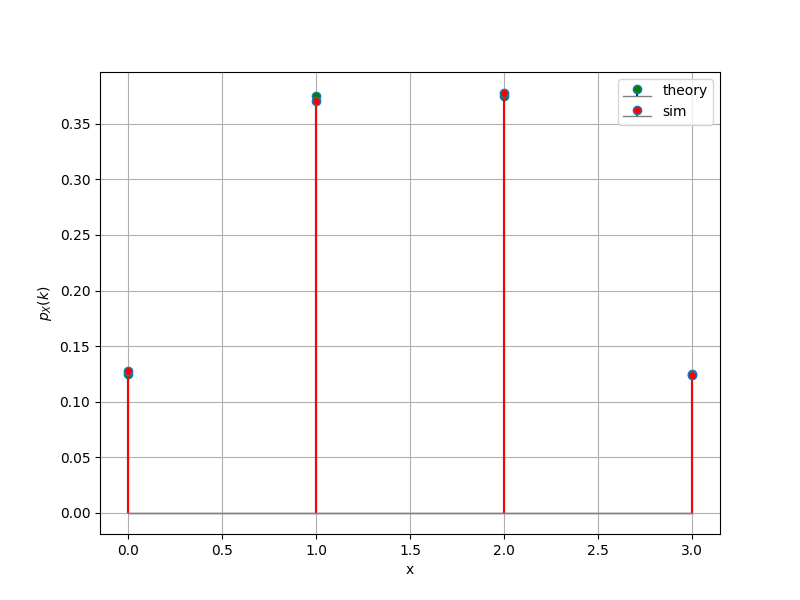
\includegraphics[width=0.8\columnwidth]{figs/pmf.png}
   \caption{PMF of the Random variable}
   \label{stemplot}
\end{figure}
\end{frame}
\begin{frame}
\begin{figure}[h!]
   \centering
   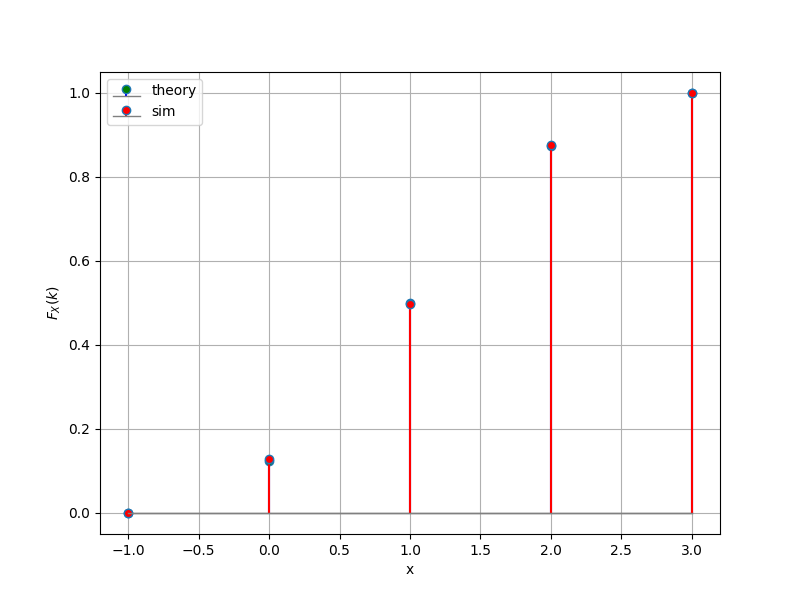
\includegraphics[width=0.8\columnwidth]{figs/cdf.png}
   \caption{CDF of the Random variable}
   \label{stemplot}
\end{figure}
\end{frame}
\begin{frame}
\begin{figure}[h!]
   \centering
   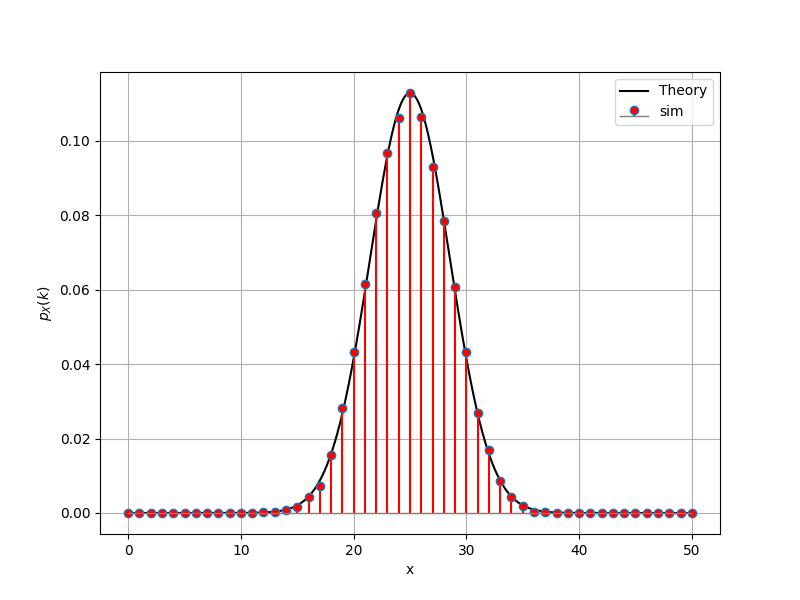
\includegraphics[width=0.8\columnwidth]{figs/gausscomp1.png}
   \caption{PMF of Binomial distribution with normal curve, n = 50, p = 0.5}
   \label{stemplot}
\end{figure}
\end{frame}
\begin{frame}
\begin{figure}[h!]
   \centering
   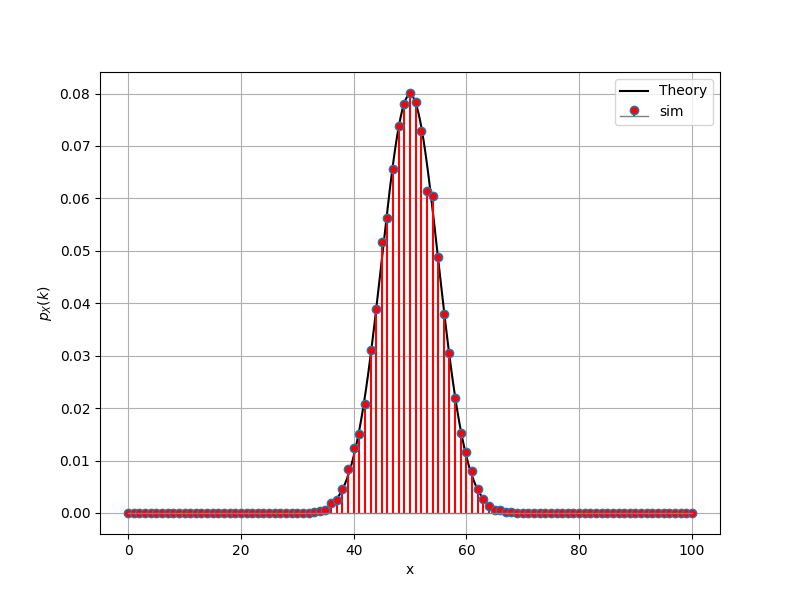
\includegraphics[width=0.8\columnwidth]{figs/gausscomp2.png}
   \caption{PMF of Binomial distribution with normal curve, n = 100, p = 0.5}
   \label{stemplot}
\end{figure}
\end{frame}
\begin{frame}
\begin{figure}[h!]
   \centering
   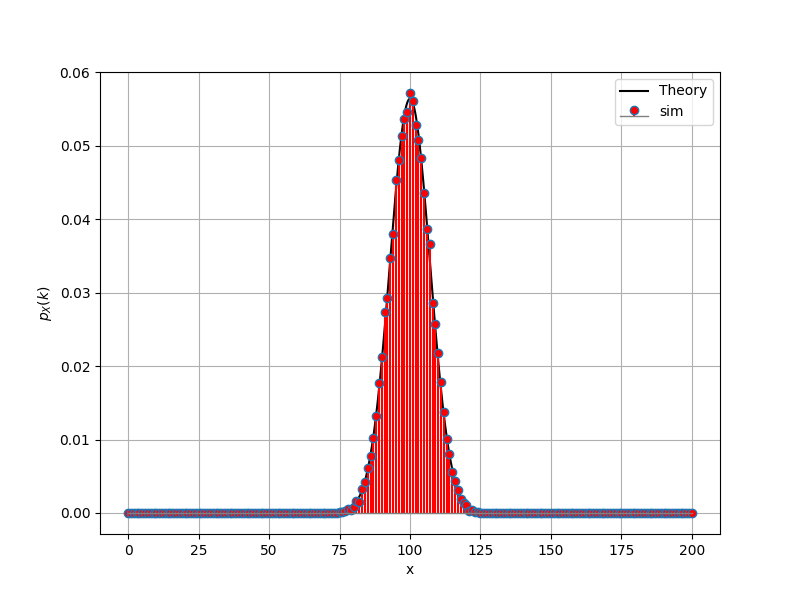
\includegraphics[width=0.8\columnwidth]{figs/gausscomp3.png}
   \caption{PMF of Binomial distribution with normal curve, n = 200, p = 0.5}
   \label{stemplot}
\end{figure}
\end{frame}
\end{document}

